\chapter{Fonctionnalités du compte}\label{chap:fonctionnalitesCompte}

\section{Menu principal}\index{menu principal|(}
\index{menu principal!liens du}

Rappelons les liens accessibles depuis ce menu situé sous l'adresse internet du site du \CdS{} et de son slogan: \liensmenu{Actualités}, \liensmenu{Membres}, \liensmenu{offres permanente}, \liensmenu{Offres}, \liensmenu{Demandes} que nous allons maintenant examiner en détails.

\subsec{Actualités}
\index{Actualites@Actualités|(}
C’est la \index{page d'accueil}page d’accueil, celle sur laquelle vous arrivez lors de la connexion (voir Fig. \ref{fig:vueGeneralePage}, p. \pageref{fig:vueGeneralePage}). Le lien \liensmenu{Actualités} permet d’y revenir à tout moment.  Y sont affichées les actualités récentes --- parfois moins récentes mais (en principe) toujours pertinentes. Dans l’exemple de la figure \ref{fig:vueGeneralePage}, apparaissent l’annonce de l’inter\sel{} qui devait avoir lieu quelques jours plus tard à Valréas, un renvoi vers le compte rendu d’un atelier récent (voir également Fig. \ref{fig:liensPertinents}, \vpageref{fig:liensPertinents}), et le début du mode d’emploi écrit par Arno (voir «~Où trouver les premières informations~», p. \pageref{page:premieresInfos}).
\begin{figure}
    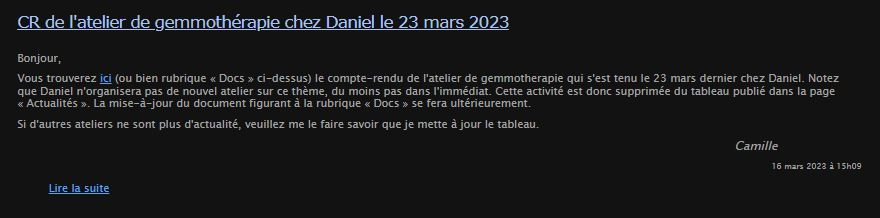
\includegraphics[width=\linewidth]{180-liens_a_cliquer_pertinents}
    \caption{Exemple de renvoi à un document depuis une actualité}
    \label{fig:liensPertinents}
\end{figure}

Cette page comporte de nombreux liens clicables sans grande utilité (voir la section <<~Autres liens~>>, p. \pageref{page:autresLiens}). \label{page:lienIci}À la figure \ref{fig:liensPertinents}, on trouve l'exemple d'un type de lien assez fréquent et qui lui, par contre, est pertinent:\index{liens vers un autre document} au début du texte le mot ici (Vous trouverez \autresliens{ici} …) est clicable et renvoie au document dont il est question, \cad{} le compte rendu de l’atelier de gemmotherapie --- plus exactement, ce lien renvoie à la rubrique \index{Docs}\liensmenu{Docs} du menu secondaire où on trouve quelques documents relatifs à notre \sel{} parmi lesquels, le compte rendu en question (nous verrons cela plus loin, p. \pageref{sec:docs}, voir également la section \og Nouveaux documents\fg dans les appendices p. \pageref{sec:nouveauxDocuments}).

\rem{\index{lien <<~Lire la suite~>>}Le lien \autresliens{Lire la suite} qui figure à la fin de toutes les actualités ne sert à rien.}
\index{Actualites@Actualités|)}

\subsec{Membres}\index{Membres|(}\label{sec:membres}

\begin{figure}
    \centering
    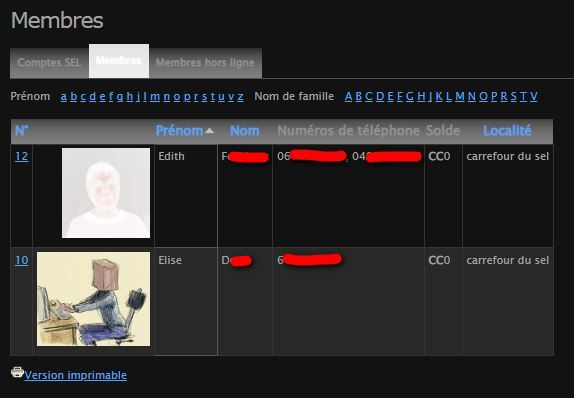
\includegraphics[width=.8\linewidth]{191-page_membres}
    \caption[Liste filtrée des membres du \CdS]{Liste filtrée (prénom commençant par <<~e~>>) des membres du \CdS}
    \label{fig:pageMembres}
\end{figure}
Cliquez sur \liensmenu{Membres} pour accéder à la page des membres actifs; un extrait de cette page est visible à la figure \ref{fig:pageMembres}. Au dessous du titre \noncliquables{Membres}, on trouve un petit menu contextuel comportant 3 liens: \liensmenu{Comptes SEL}, \liensmenu{Membres} et \liensmenu{Membres hors ligne}.

Passons rapidement sur le premier et le troisième lien qui ne nous intéressent guère. Sous le premier, \liensmenu{Comptes SEL}%
%%%
\footnote{Voir la section \og Notion de rôle\fg, p. \pageref{sec:responsabilitesSite} }
%%%
\index{Membres!Comptes SEL}, on trouve des membres liés à la création du site (et qui peuvent être extérieurs au \sel) et sous le troisième, \liensmenu{Membres hors-ligne}\index{Membres!hors ligne}, les membres qui ne n’ont pas de connexion à internet --- cinq adhérentes et un adhérent sont dans ce cas à l’heure actuelle%
%%%
\footnote{Un système de parrainage ou de marrainage est mis en place pour que ces adhérentes et cet adhérent soient tenu(e)s au courant des activités.}.
%%%

Sous le deuxième onglet, vous trouverez la liste des membres actifs\index{Membres!actifs, liste des}%
%%%
\footnote{Sous réserve que les dernières mises à jour soient faites car il  y a parfois un petit décalage surtout à l’époque des renouvellements.}.
%%%
Les listes de lettres suivant les intitulés \noncliquables{Prénom} et \noncliquables{Nom de famille} permettent d’affiner la sélection. À la figure \ref{fig:pageMembres}, on a cliqué sur <<~e~>> dans la liste des prénoms et seuls les membres dont le prénom commence par «~E~» sont sélectionnés --- en fait,  <<~E~>> ou <<~É~>> car les accents sont ignorés.

Les colonnes sont les suivantes: 
\begin{enumerate}
    \item \index{numero de membre@numéro de membre}numéro de membre (il s’agit du numéro d’enregistrement sur le site et non du numéro du carnet d’échange papier remis à chaque membre);
    \item photo de l’adhérent(e)\index{photo!de profil};
    \item nom de famille\,;
    \item numéro(s) de téléphone;
    \item le solde (du compte) n’est pas utilisé au \CdS;
    \item sel d’appartenance (depuis la mise en sommeil du Sel des 3 Rivières et du Galet du Buech, il ne subsiste plus que le \CdS).
\end{enumerate}
La photo n'est présente que si elle a été ajoutée par le membre (voir section <<~Ajouter une photo de profil~>>, p. \pageref{sec:insererImage}).

\rem{Pour le lien \autresliens{Version imprimable}, voir la section \og Nouveaux documents\fg dans les appendices (p. \pageref{sec:nouveauxDocuments}).}

\ssubsec{Accéder à la fiche de profil d'un membre}
\label{sec:ficheProfil}
\index{fiche de profil|(}

\begin{figure}
    \centering
    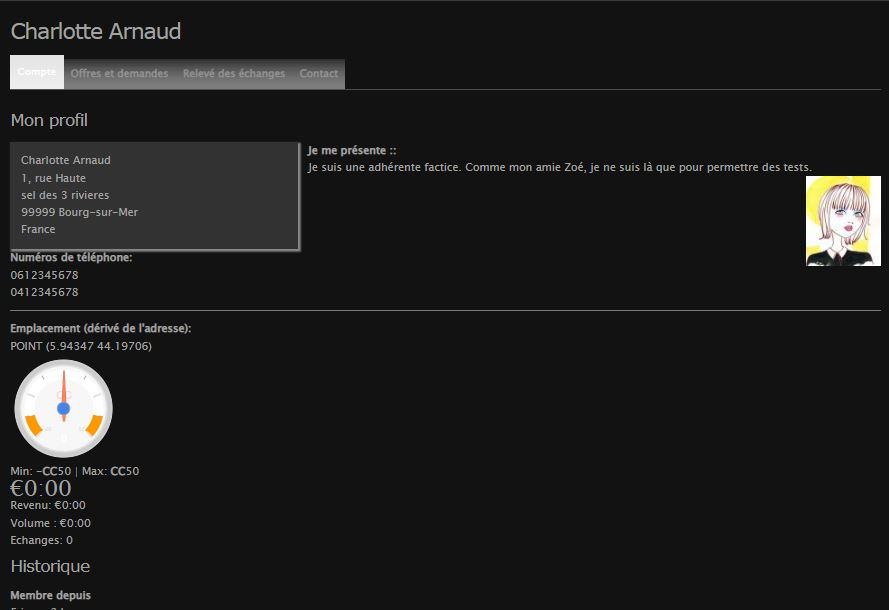
\includegraphics[width=.9\linewidth]{201-fiche_membre}
    \caption[Fiche de profil de Charlotte \textsc{Arnaud}]{Fiche de profil de Charlotte \textsc{Arnaud} telle que vue par un autre membre}
    \label{fig:ficheMembre}
\end{figure}
\begin{figure}
    \centering
    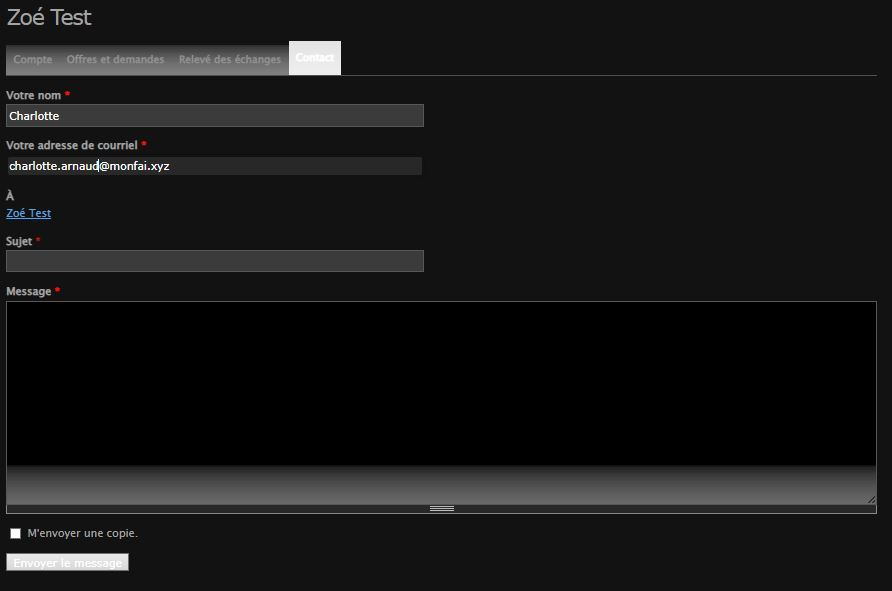
\includegraphics[width=.9\linewidth]{210-message_a_zoe}
    \caption[Formulaire de contact]{Formulaire de contact (envoyer un message à un autre membre)}
    \label{fig:envoiMessage}
\end{figure}
Le \index{numero de membre@numéro de membre}numéro de membre de la colonne 1 est clicable, il permet d’accéder à la fiche de profil du membre --- il est également possible de cliquer sur le cadre photo, que celle-ci soit présente ou non, avec le même résultat. Voici à la figure \ref{fig:ficheMembre} la fiche de l'utilisatrice factice qui nous accompagne dans ce tutoriel.

Vous observerez que la figure \ref{fig:ficheMembre} (\vpageref{fig:ficheMembre}) ressemble beaucoup celle de la figure \ref{fig:monCompteVoir} (p. \pageref{fig:monCompteVoir}); en effet, dans les deux cas il s'agit de la fiche de profil de Charlotte mais vue par Charlotte elle-même à la figure \ref{fig:monCompteVoir} et vue par un autre membre à la figure \ref{fig:ficheMembre}%
%%%
\footnote{La fiche de profil d'un membre \og hors ligne\fg et un peu différente, voir la section \og Page profil d'un membre  "hors ligne"\fg" dans les appendices (p. \pageref{sec:profilMembreHorsLigne}).}.

Le menu contextuel est différent selon la fiche est vue par Charlotte ou par un autre membre:
\begin{itemize}
    \item Lorsque Charlotte est sur sa propre fiche, le lien \liensmenu{Compte} du menu contextuel ouvre un sous-menu qui lui permet de modifier ses informations. Nous avons vu cela au chapitre \ref{chap:personnaliserCompte} <<~Personnaliser votre compte~>>.
    \item Lorsque la fiche de Charlotte est consultée par un autre membre ce sous-menu n'apparaît pas car un autre membre n'a pas le droit de modifier les informations de Charlotte%
    %%%
    \footnote{À l'exeption des administrateurs locaux (voir section \og{}Administrateur local\fg{}, p. \pageref{sec:adminLocal}) p.ex. pour réinitialiser votre mot de passe si nécessaire (voir <<~Mot de passe oublié~>>, p. \pageref{sec:mdpOublie}).}.
    %%%
    Par contre, le menu contextuel comporte un lien \liensmenu{Contact} supplémentaire (voir ci-après).
\end{itemize}
\index{fiche de profil|)}

\ssubsec{Envoyer un message à un autre membre}\label{page:envoyerCourrielMembre}\index{envoyer un message}
\index{contacter!un autre membre}

La figure \ref{fig:envoiMessage} \vpageref{fig:envoiMessage} montre ce qu’obtient Charlotte lorsqu’elle clique sur le lien \liensmenu{Contact} de Zoé%
%%%
\footnote{Zoé est une autre adhérente factice; elle est parfois utilisée pour réaliser certains tests. Comme Charlotte, Zoé est  au \sel{} des 3 Rivières.}.
%%%
Il s’agit d’un formulaire de contact très classique qui n’appelle pas de longues explications. Deux des quatre champs obligatoires (astérisque rouge) sont pré-remplis, \noncliquables{Votre nom} et \noncliquables{Votre adresse courriel}, les deux autres sont les champs \noncliquables{Sujet} et \noncliquables{Message}.

Si vous voulez recevoir une copie, n'oubliez pas de cocher la case prévue, puis, bien sûr, cliquez sur \autresliens{Envoyer le message}.
 
\rem{Notez que  lorsque Zoé recevra ce message elle connaîtra l’adresse courriel de Charlotte%
%%%
\footnote{Dans le champ \og{}Répondre à\fg.};
%%%
elle pourra lui répondre sans passer par le site.}
\index{Membres|)}

\subsec{Offres permanentes, Offres, Demandes}

Les trois derniers onglets sont assez semblables, nous allons les voir ensemble.
\index{offres!différents types!ponctuelle}
\index{offres!différents types!permanente}
\label{page:typesOffres}Rappelons d’abord la différence entre \liensmenu{Offres} et \liensmenu{Offres permanentes}. Cette dernière catégorie a été ajoutée spécifiquement pour le site du \CdS{} à notre demande. Une offre permanente, contrairement à une offre simple ou offre ponctuelle, n’a pas de limite dans le temps. Si vous proposez un covoiturage pour une exposition à Marseille samedi prochain, cette offre est caduque dès samedi prochain, il s’agit d’une offre ponctuelle. Si vous proposez une aide à l’utilisation de la bureautique, l’offre est probablement permanente.

L'intitulé de ces liens est assez explicite, ils permettent d’ouvrir les pages correspondantes: listes des offres permanentes, des offres (ponctuelles) et des demandes. 

\ssubsec{Offres ponctuelles et demandes}

\index{offres!consulter les|(}
\index{demandes!consulter les|(}
La figure \ref{fig:offresDebut} montre le début de la liste d’offres et la figure \ref{fig:demandesFin} la fin de la liste de demandes. Ces deux listes comportent au début un petit menu contextuel mais seul le premier lien \liensmenu{Tout} est utile, les deux autres, \liensmenu{Offre/demande ponctuelle} et \liensmenu{Offre/demande permanente}%
%%%
\footnote{D'ailleurs, la catégorie demande permanente n'existe pas!},
%%%
renvoient à une page vide.
\begin{figure}
    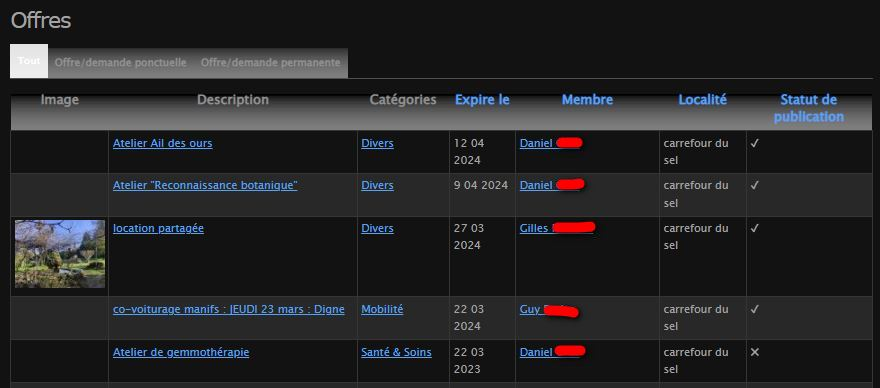
\includegraphics[width=\linewidth]{221-liste_offres_debut}
    \caption[Liste des offres]{Liste des offres (début de la liste)}
    \label{fig:offresDebut}
\end{figure}
\begin{figure}
    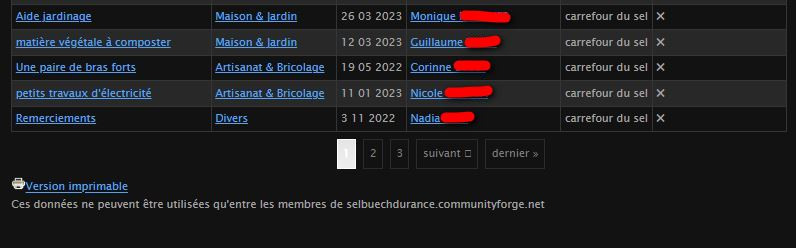
\includegraphics[width=\linewidth]{231-liste_demandes_fin}
    \caption[Liste des demandes]{Liste des demandes (fin de la liste)}
    \label{fig:demandesFin}
\end{figure}

Les deux listes comportent 7 colonnes\,:
\begin{enumerate}
    \item une image \index{image!transférer}téléchargée par l’auteur de l’offre/demande (rarement utilisée pour une demande mais peut être très utile pour une offre);
    \item une courte description de l'offre/demande, en cliquant sur cette colonne vous devriez accéder à une description plus complète%
    %%%
    \footnote{Si, du moins, l'auteur(trice) de l'annonce a fourni cette description détaillée ; il est (fortement) conseillé de le faire mais ce n'est pas obligatoire (voir section \og{}Texte de l'annonce\fg, p. \pageref{sec:texteAnnonce}).};
    %%%
    \item la catégorie de l'offre/demande\footnote{Un certain nombre de catégories sont actuellement disponibles (voir Fig. \ref{fig:categories_offres}, p. \pageref{fig:categories_offres}) mais elles pourront à l’avenir être modifiées. Si une nouvelle catégorie vous paraît nécessaire, prenez contact avec moi.}, en cliquant sur la catégorie vous obtiendrez la liste de toutes les offres/demandes de cette même catégorie;
    \item la date d’expiration telle qu’elle a été définie par l’auteur(trice) de l’offre/demande (nous y reviendrons à la section <<~Durée de validité de l’annonce~>>, p. \pageref{sec:dureeValiditeAnnonce});
    \item l’identité du membre qui a publié l’offre/demande, en cliquant sur son nom on accède à sa fiche pour, notamment, prendre contact avec lui (voir la section <<~Envoyer un message à un autre membre~>>, p. \pageref{page:envoyerCourrielMembre});
    \item la localité du membre --- à ce jour, tous les membres (réels) sont au \CdS;
    \item le statut de publication, à la figure \ref{fig:offresDebut} les 4 premières annonces sont encore publiées (symbole \ding{52}), la cinquième ne l’est plus, l’atelier ayant eu lieu (symbole \ding{53}), de même, toutes les demandes de la fin de liste à la figure \ref{fig:demandesFin} sont périmées (\ding{53})
\end{enumerate}

À la figure \ref{fig:demandesFin}, on trouve un lien intitulé \autresliens{Version imprimable} qui permet de générer un fichier au format \termecode{pdf} de la liste que vous pouvez facilement imprimer. Ce lien est également présent à la fin de la liste des offres\footnote{Ces listes comportent toutes les annonces qui n'ont pas été effacées d'où l'importance d'effacer les annonces périmées ce que, hélas, peu de gens font ! (voir la section <<~Durée de validité de l'annonce~>> \vpageref{sec:dureeValiditeAnnonce})}.
\index{demandes!consulter les|)}

\ssubsec{Offres permanentes}

La liste des offres permanentes est assez semblable aux deux précédentes sauf qu’il n’y a que 5 colonnes --- localité et statut de publication sont absents%
%%%
\footnote{La localité n'est guère utile dans notre cas puisqu'il n'y en a qu'une, le \CdS. C'est un peu la même chose pour le statut de publication car une offre permanente est normalement publiée ... en permanence, et si elle n'a plus cours elle doit être \index{annonce!supprimée}supprimée et non \index{annonce!dépubliée}dépubliée (à nouveau, voir ci-après la section <<~Durée de validité de l'annonce~>> \vpageref{sec:dureeValiditeAnnonce}): donc le statut de publication est nécessairement <<~Publié~>>.}
%%%
--- et dans un ordre  différent.

Malheureusement, la principale différence est que le lien \autresliens{Version imprimable} n'y figure pas alors que c’est pour cette liste qu’il serait le plus utile\,!
\index{offres!consulter les|)}\index{menu principal|)}

\section{Menu secondaire}
\index{menu secondaire|(}
\index{menu secondaire!liens du}

Ce menu situé en haut à droite des pages comporte, rappelons-le, les liens suivants: \liensmenu{Docs}, \liensmenu{FAQ}, \liensmenu{Contact}, \liensmenu{Albums}, et \liensmenu{Politique de confidentialité} (ou RGPD).

Passons rapidement sur les liens \liensmenu{FAQ} --- dont nous avons parlé dans la première partie (voir la section \og{}Où trouver les premières informations\,?\fg, p. \pageref{page:premieresInfos}) ---, et \liensmenu{Contact}\index{contacter!responbles} qui permet, à l'aide d'un menu déroulant, de contacter les différents responsables de l'association par catégorie (<<~Demande d'information~>>, <<~Comptabilité~>>, etc.); ce lien n’est pas très utile pour les adhérent(e)s, contactez directement Jacqueline ou Mathieu
 --- ou encore moi s'il s'agit de l'utilisation du site \CF.
 \rem{Si toutefois vous voulez passer par ce lien, sachez que seule la rubrique \og{}Demande d’information\fg est fonctionnelle et que le message est envoyé à Jacqueline et à Mathieu%
 %%%
 \footnote{S'il est de peu d'intérêt pour les membres que nous sommes, ce lien est utile pour les visiteurs}.}

Nous passerons rapidement aussi sur le lien \liensmenu{Albums}\index{Album de photos}. Il est possible de déposer sur le site des photos liées à l’activité du \sel{} (ou pas), réparties dans différents albums. Depuis le départ d’Arno, cette rubrique est à l’abandon. Les photos qui apparaissent dans le bloc \noncliquables{Une photo au hasard}\index{photo!au hasard} --- si vous ne l’avez pas supprimé (voir section <<~Supprimer l'affichage de certains blocs~>>, p. \pageref{sec:supprimerBlocs}) --- sont tirées de celles qu’il avait téléchargées à l’époque.

\rem{Si vous souhaitez vous impliquer pour  redonner vie à cette rubrique, prenez contact avec un membre du comité (voir liste p. \pageref{sec:comite}.) car seuls ces membres peuvent créer et alimenter les albums.}

\subsec{Politique de confidentialité (RGPD)}\label{sec:rgpd}
\index{RGPD|(}
Les sites de \CF, et donc celui du \CdS, sont certifiés compatibles RGPD (Règlement Général sur la Protection des Données). Le lien \liensmenu{Politique de confidentialité} permet d’accéder à une page qui précise les engagements de \CF{} vis-à-vis du RGPD. En particulier, \CF{} vous garantit que les informations de votre \index{fiche de profil}page de profil ne seront jamais divulguées publiquement.
Plus généralement, à propos du RGPD, vous pouvez consulter le site de la \textsc{Cnil}\index{Cnil@\textsc{Cnil}}:

\smallskip

\begin{center}
    \liensdirects{https://www.cnil.fr/fr/rgpd-de-quoi-parle-t-on}
\end{center}

\smallskip

Si vous n’avez pas pris connaissance de vos droits et obligations en lien avec le RGPD lorsque vous avez signifié votre acceptation, il est temps de le faire --- voir la section sur l'activation du compte au chapitre \ref{chap:premiersPas} (notamment p. \pageref{page:accepteRgpd}). 
\TCBimportant{\label{enc:nePasDivulguer}Le point le plus important est qu'il ne faut en aucun cas divulguer à l'extérieur les informations publiées sur ce site; elles ne doivent être accessibles qu'aux adhérent(e)s --- notamment le contenu des \index{fiche de profil}pages de profil.
\aster
    Attention, si vous le faites, votre responsabilité peut se trouver engagée devant un tribunal.
}
\index{RGPD!|)}

\subsec{Docs}\label{sec:docs}
\index{Docs|(}

\begin{figure}
    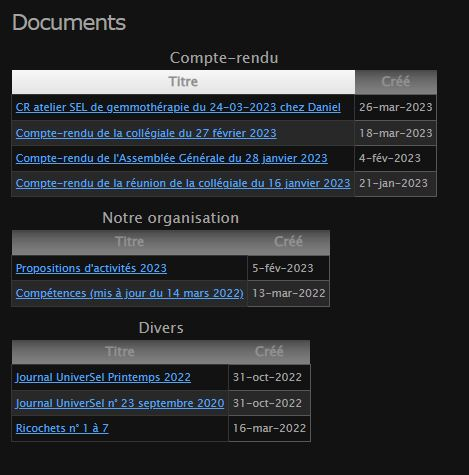
\includegraphics[width=\linewidth]{240-page_docs}
    \caption[Liste des documents]{Liste des documents (juin \oldstylenums{2023})}
    \label{fig:listeDocuments}
\end{figure}
Nous avons déjà brièvement évoqué le lien \liensmenu{Docs} au chapitre \ref{chap:premiersPas}, section «~Où trouver les premières informations\,?~» (p. \pageref{page:premieresInfos}). Ce lien amène sur une page où sont listés des documents permanents concernant la vie du \sel, classés par catégorie.
\rem{Seuls les membres du comité peuvent sauvegarder des documents (voir la liste à section <<~Comité~>>, p. \pageref{sec:comite}). Si besoin, faites appel à l'un d'eux.}

La figure \ref{fig:listeDocuments} (\vpageref{fig:listeDocuments}) montre les documents disponibles à la date de la capture d'écran. Ils sont encore peu nombreux, espérons que cette rubrique s’étoffera dans l’avenir car ces documents, contrairement aux annonces et aux actualités, sont permanents: ils témoignent donc de l'activité du \sel. À terme, le présent texte sera archivé dans une rubrique <<~Tutoriels~>> vide pour l'instant.

On accède aux documents de deux  façons différentes.

On peut le faire  en cliquant sur le lien \liensmenu{Docs} du menu secondaire --- ce qui ouvre la fenêtre de la figure \ref{fig:listeDocuments} ---, puis en cliquant sur le document souhaité, p.ex. \autresliens{Propositions d’activités 2023}. Le résultat de ce clic dépend du format du fichier sauvegardé. S’il s’agit d’un document au format \termecode{pdf}, il s’ouvrira automatiquement dans la plupart des navigateurs, dans d’autres cas, p.ex. un document au format \termecode{docx}, il faudra souvent l’enregistrer d'abord sur son ordinateur pour ensuite l’ouvrir avec le logiciel approprié --- Microsoft Office ou LibreOffice ou OpenOffice dans le cas d’un \termecode{docx}. 

Privilégiez donc le format \termecode{pdf} lorsque vous proposez des documents à archiver cela en facilitera la lecture pour les autres membres.

Mais on peut aussi accéder à certains documents depuis un lien publié ailleurs, notamment dans la page \noncliquables{Actualités} (voir p. \pageref{page:lienIci} et Fig. \ref{fig:liensPertinents}, p. \pageref{fig:liensPertinents}).
\index{Docs|)}\index{menu secondaire|)}

\section{Menu utilisateur}
\label{sec:menuUtilisateur2}
\index{menu utilisateur|(}
\index{menu utilisateur!liens du}

Ce menu (voir p. \pageref{fig:menuUtilisateur}) comporte les liens suivants:  \liensmenu{Mon compte}  vu au chapitre \ref{chap:personnaliserCompte} <<~Personnaliser votre compte~>> (p. \pageref{chap:personnaliserCompte} et suivantes), \liensmenu{Saisir un échange} qui n'est pas utilisé au \CdS, \liensmenu{Se déconnecter} dont la signification est évidente, \liensmenu{Enregistrer une offre ponctuelle} et \liensmenu{ajouter une offre permanente} (pour la différence entre offre permanente et ponctuelle voir \vpageref{page:typesOffres}), \liensmenu{Enregistrer une demande} et enfin \liensmenu{Ajouter du contenu}. Dans cette section, nous allons voir les quatre derniers.

\subsec{Enregistrer une offre ponctuelle}
\index{annonce!offre ponctuelle|(}

\ssubsec{Texte de l'annonce}\label{sec:texteAnnonce}
\index{annonce!offre ponctuelle!rédaction du texte|(}

\begin{figure}
    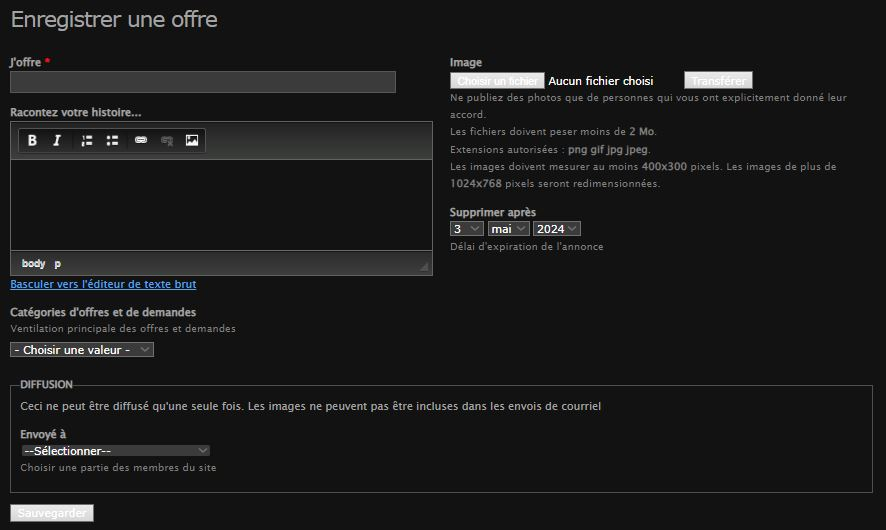
\includegraphics[width=\linewidth]{250-enregistrer_offre}
    \caption{Page d’enregistrement d’une offre}
    \label{fig:enregisterOffre}
\end{figure}
Le lien \liensmenu{Enregistrer une offre ponctuelle} ouvre la page de la figure \ref{fig:enregisterOffre}. Le champ \noncliquables{J’offre} est le seul obligatoire. Évitez les textes trop vagues; si vous écrivez, p.ex., «~Tomates~», cela signifie-t-il que vous proposez des tomates, des plants de tomates, autre chose\,? <<~Offre tomates vertes pour confiture~>> sera beaucoup plus informatif\,!

Le champ \noncliquables{Racontez votre histoire ...} permet d’ajouter des informations utiles, \ex, pour des plants de tomates, les variétés, s'il s'agit de godets ou de racines nues, comment les récupérer, etc. Ce champ n'est pas obligatoire mais il est fortement conseillé de le remplir --- et de le faire avec soin --- pour la qualité des échanges.

\index{RGPD|(}
\TCBimportant{Mais n'indiquez jamais de \index{donnees personnelles@données personnelles}données personnelles dans le texte d'une annonce (adresse, numéro de téléphone, adresse courriel, etc.)\,! \CF{} garantit la confidentialité des informations contenues dans votre \index{fiche de profil}page de profil (voir la section <<~Politique de confidentialité~>> p. \pageref{sec:rgpd}), pas de celles figurant explicitement dans une annonce qui sont, elles, visibles publiquement (Fig. \ref{fig:donnees_personnelles_compromises}).}

\begin{figure}[h]
    \centering
    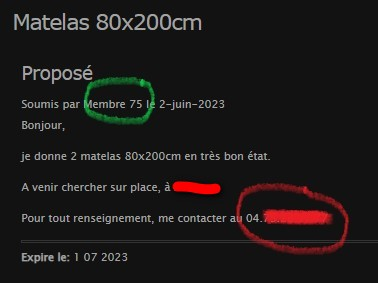
\includegraphics[width=.6\linewidth]{264-annonce_a_ne_pas_faire}
    \caption{Exemple d'annonce compromettant des \index{donnees personnelles@données personnelles}données personnelles}
    \label{fig:donnees_personnelles_compromises}
\end{figure}

\index{donnees personnelles@données personnelles|(}Cette figure montre une annonce telle que la voit un visiteur du site: le nom du membre a bien été anonymisé (membre 75) mais l'auteur ou l'autrice de cette annonce a indiqué son numéro de téléphone dans le contenu de l'annonce, celui-ci ne pouvant pas être anonymisé, le numéro se trouve exposé publiquement. La formulation correcte consiste à indiquer seulement: <<~Pour tout renseignement, me contacter~>> et lorsque cette annonce est vue par un(e) adhérent(e), <<~membre XX~>> est remplacé par le nom de ce membre, (\ex) Charlotte \textsc{Arnaud}; les membres intéressés pas l'annonce peuvent alors se reporter à la \index{fiche de profil}page de profil de Charlotte (voir section <<~Accéder à la fiche de profil d'un membre~>>, p. \pageref{sec:ficheProfil}) pour connaître ses coordonnées, en particulier téléphoniques%
%%%
\footnote{Ou bien utiliser le formulaire de contact (voir section <<~Envoyer un message à un autre membre~>>, p. \pageref{page:envoyerCourrielMembre})}.
%%%
\rem{Depuis la capture d'écran de la figure
\ref{fig:enregisterOffre}, 
j'ai demandé à \CF{} d'ajouter un petit avertissement\footnote{Sur la suggestion d'\'Eric Le Chaix de \sel'idaire.} 
à la suite de \noncliquables{Racontez votre histoire ...} qui est devenu \noncliquables{Racontez votre histoire... Mais, ici ne laissez pas de données personnelles (RGPD) : mail, tel, adresse...},
rappelant qu'il ne faut pas laisser de données 
personnelles dans les annonces.

\medskip

\begin{mybox}[colbacktitle=MidnightBlue]{À propos du RGPD (suite)}
    La raison d'être du RGPD est de protéger les citoyens européens des risques encourus lorsque des informations personnelles sont divulguées publiquement: arnaque, usurpation d'identité, harcèlement, etc., la liste est longue. Les victimes peuvent être les personnes dont les informations ont fuitées mais aussi leurs ayants droit.
    \aster
    Les administrateurs de sites internet sont responsables de la conformité du site au RGPD et ils peuvent être mis en cause en cas de dommages s'ils n'ont pas pris les mesures nécessaires pour assurer cette conformité. Pour les sites \CF{}, ils doivent notamment s'assurer que les annonces qui sont visibles publiquement ne contiennent pas de données personnelles et, le cas échéant, les \index{annonce!supprimée}supprimer.
    \aster
    Au \CdS{} où il n'y a pas de contrôle a priori de contenu des annonces, ces informations seront \index{annonce!supprimée}supprimées dès que possible mais il est préférable que chacune et chacun évite tout problème en amont, dès la rédaction de l'annonce. 
\end{mybox}
\index{donnees personnelles@données personnelles|)}
\index{RGPD|)}}

\medskip
\index{annonce!mise en forme du texte|(}
Le champ \noncliquables{Racontez votre histoire ... } offre quelques outils de mise en forme, assez peu nombreux mais souvent suffisants: vous pouvez mettre du gras, de l’italique, insérer des listes numérotées ou non, ajouter ou supprimer un lien et enfin insérer une image (toutefois, préférez pour cela les images externes au texte, voir la section suivante <<~Insérer une image~>>). Si vous maîtrisez le langage \termecode{html}, vous pouvez cliquer sur le lien \autresliens{Basculer vers l’éditeur de texte brut}\index{editeur de texte brut@éditeur de texte brut}\label{page:editeurTexteBrut} ce qui vous donnera à accès plus de possibilités de mise en forme%
%%%
\footnote{Mais ne vous attendez pas à trouver les outils qu'offrent généralement les éditeurs de code tels que coloration syntaxique, complétion, etc. Selon mon expérience personnelle, mieux vaut préparer son texte localement avec un vrai éditeur de code (notepad++ pour un des plus simples, Visual Studio Code, Emacs, etc.) et faire ensuite un copié/collé. Pour autant, toutes les balises ne vous seront pas autorisées, notamment la dangereuse balise \termecode{script} sera désactivée.}.
%%%
\index{annonce!mise en forme du texte|)}
\index{annonce!offre ponctuelle!rédaction du texte|)}

\ssubsec{Insérer une image}\index{image!transférer}
\index{annonce!offre ponctuelle!ajouter une image|(}

Si vous proposez, \ex{} une table, c’est peut-être une bonne idée d’ajouter une photo de cette table à votre annonce.\index{image!transférer} Pour cela, cliquez sur \autresliens{Choisir un fichier} ce qui ouvre une fenêtre sur votre terminal, naviguez jusqu’à l’image à insérer, cliquez sur \autresliens{Ouvrir}, et finalement  cliquez sur le lien \autresliens{Transférer}. Notez que cette procédure peut varier selon votre système d’exploitation (Windows, Apple, Linux). Pour le choix de l’image, respectez les consignes qui apparaissent à l’écran (dimensions, taille du fichier, etc.), \textbf{sans oublier l'accord des personnes s’il y a lieu}.
\index{annonce!offre ponctuelle!ajouter une image|)}

\ssubsec{Durée de validité de l'annonce}\label{sec:dureeValiditeAnnonce}
\index{annonce!offre ponctuelle!définir durée de validité|(}

Le champ date \noncliquables{Supprimer après} permet de limiter la durée de validité de l’annonce. Par défaut, elle est de 3 mois mais cette durée est rarement pertinente. Si vous proposez une sortie pour le mois prochain, inutile de laisser l'annonce active pendant 3 mois. N’oubliez donc pas de préciser à quelle date elle doit être désactivée --- ou de la désactiver vous-même si elle cesse d'être valide avant cette date.

Prenons quelques exemples pour clarifier les choses\,:
\begin{enumerate}
    \item Le \oldstylenums{1}\ier mai, vous proposez une randonnée pour le \oldstylenums{7} du même mois, indiquez le \oldstylenums{7} mai, ou à la rigueur le \oldstylenums{8}, comme date de suppression%
    %%%
    \footnote{Il y a une certaine confusion entre suppression et désactivation de l'annonce, voir le paragraphe ci-après.}.
    %%%
    \item  Vous demandez des plants de tomates, si vous ne les avez pas obtenus d'ici 3 ou 4 semaines, vous n'en avez probablement plus besoin, indiquez donc un délai pour la désactivation de 3/4 semaines et, si vous obtenez les plants dans les 48h, \index{annonce!dépubliée}dépubliez/\index{annonce!supprimée}supprimez l'annonce immédiatement.
    \item Dernier exemple, vous avez besoin d'aide (un brigadou) pour ranger le fatras accumulé depuis des années dans votre grenier: vous pouvez porter le délai de validité à 6 mois, voire 1 an et dès que votre grenier sera rangé, \index{annonce!supprimée}supprimez l'annonce.
\end{enumerate}
\rem{Les exemples 2 \& 3 sont des demandes plutôt que des offres mais le principe est le même.}

Contrairement à ce que suggère le libellé \noncliquables{Supprimer après}, l'annonce n'est pas réellement \index{annonce!supprimée}supprimée, elle est seulement \index{annonce!dépubliée} dépubliée \cad qu'elle cesse d'être visible par les autres membres mais elle est toujours présente dans la base de données du site et vous pouvez accéder à vos propres annonces \index{annonce!dépubliée} dépubliées depuis le  menu utilisateur, onglet \liensmenu{Mon compte} puis \liensmenu{Offres et demandes} du menu contextuel  (voir \vpageref{page:compte_offres_demandes}).

\begin{figure}
    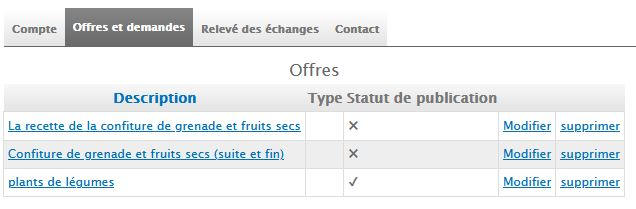
\includegraphics[width=\linewidth]{147-mon_compte_offres_et_demandes}
    \caption[Onglet <<~Offres et demandes~>> du lien <<~Mon compte~>> dans le menu utilisateur]{Onglet \liensmenu{Offres et demandes} du lien \liensmenu{Mon compte} dans le menu utilisateur}
    \label{fig:compte_offres_demandes}
\end{figure}
Comme Charlotte \textsc{Arnaud} s'est abstenue de publier des annonces qui n'auraient pu être que fantaisistes, l'illusration de la figure \ref{fig:compte_offres_demandes} provient des annonces d'un utilisateur réel. On y trouve le statut de publication, publiée (\ding{51}) ou \index{annonce!dépubliée}dépubliée (\ding{53}) de l'annonce mais surtout deux liens \index{annonce!modifiée}\autresliens{Modifier} et \index{annonce!supprimée}\autresliens{supprimer} permettant, ainsi que le nom l'indique, de \index{annonce!modifiée}modifier --- et si besoin de \index{annonce!republiée}republier ---, ou de \index{annonce!supprimée}supprimer l'annonce. Comme la plupart du temps les annonces \index{annonce!dépubliée}désactivées n'ont pas vocation à être réutilisées, il est préférable de venir sur cet onglet pour les \index{annonce!supprimée}supprimer complètement plutôt que simplement les \index{annonce!dépubliée}déactiver. Donc, dans les exemples ci-dessus, lorsque la randonnée est terminée et le grenier rangé, \index{annonce!supprimée}supprimez l'annonce, et sans doute également lorsque vous n'avez plus besoin des plants de tomates  --- il est trop tard pour les planter, vous les avez obtenus par ailleurs, etc.\rem{Je fais de temps en temps le ménage pour \index{annonce!supprimée}supprimer les (très) vieilles annonces manifestement à l'abandon mais il vaudrait mieux que ce travail soit fait par l'auteur ou l'autrice, c'est lui ou elle qui sait le mieux si son annonce doit être \index{annonce!dépubliée}désactivée ou \index{annonce!supprimée}supprimée, ou si elle doit être conservée%
%%%
\footnote{Si vous avez des annonces que vous souhaitez conserver au-delà de la date de \index{annonce!dépubliée}désactivation, faites-le moi savoir.}!}

    % \begin{wrapfigure}[10]{L}{.3\linewidth}
    %     \centering
    %     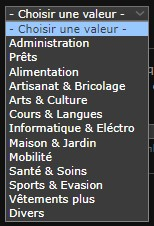
\includegraphics[width=.75\linewidth]{255-categories_offres}
    %     \caption{Catégorisation des offres}
    %     \label{fig:categories_offres}
    % \end{wrapfigure}

    \index{annonce!offre ponctuelle!définir durée de validité|)}

    \ssubsec{Catégorisation}
    \index{annonce!offre ponctuelle!indiquer la catégorie|(}

    \begin{figure}
        \centering
        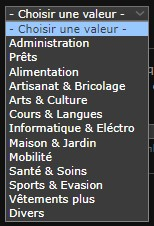
\includegraphics[width=.3\linewidth]{255-categories_offres}
        \caption{Catégorisation des offres}
        \label{fig:categories_offres}
    \end{figure}
    
Dans le menu déroulant intitulé \noncliquables{Choisir une valeur} indiquez la catégorie de votre annonce. La figure \ref{fig:categories_offres} liste les catégories disponibles; celles-ci peuvent être modifiées. Si vous pensez qu'une catégorie devrait être ajoutée, contactez-moi.
\index{annonce!offre ponctuelle!indiquer la catégorie|)}


\ssubsec{Sauvegarde et diffusion}
\label{sec:sauvegarder_diffuser}
\index{annonce!offre ponctuelle!enregistrer et diffuser|(}

\label{page:choixLocalite}
Finalement, il vous faut décider de l'option de diffusion. Attention, si vous vous contentez de cliquer sur le lien \autresliens{Sauvegarder}, votre annonce sera simplement … sauvegardée, \cad{} qu’elle apparaîtra bien sur le site mais aucun courriel ne sera envoyé. En général, ce n’est pas ce que vous voulez%
%%%
\footnote{Une exception est lorsque vous voulez juste apporter une \index{annonce!modifiée}modification à votre annonce sur le site sans la rediffuser --- nous avons vu à la section  <<~Durée de validité de l'annonce~>> \vpageref{sec:dureeValiditeAnnonce} comment modifier une annonce.},
%%%
ce que vous voulez c’est que les adhérent(e)s reçoivent le texte de l’annonce. Pour cela, il faut indiquer une valeur dans le menu déroulant du champ \noncliquables{Envoyé à}. Depuis la mise en sommeil des \sel{} de Sisteron et  Laragne, ces deux localités ont été supprimées, reste donc \autresliens{Tous les autres adhérents actifs} et \autresliens{Tous ceux de ma localité}; la différence entre les deux est que avec \autresliens{Tous ceux de ma localité} les deux adhérentes factices, Charlotte et Zoé, qui sont membres du \sel{} des 3 Rivières, ne seront pas destinataires du message, c'est donc le bon choix%
%%%
\footnote{Si vous choisissez \autresliens{Tous les autres adhérents actifs}, ce n'est pas très grave mais c'est à éviter car l'adresse électronique provisoire utilisée pour créer le compte de Charlotte \textsc{Arnaud} --- dont j'ai encore besoin quelques temps --- n'est plus valide, or \CF nous demande d'éviter les adresses incorrectes.}.
%%%
La dernière possibilité, \autresliens{Juste à moi},  peut être utile quelquefois pour faire un test avant une diffusion générale. 

Un fois le paramètre de diffusion sélectionné, le bouton \autresliens{Sauvegarder} devient \autresliens{Sauvegarder et diffuser}, il ne vous reste plus qu'à cliquer dessus.
\index{annonce!offre ponctuelle!enregistrer et diffuser|)}

\medskip

\begin{mybox}[colbacktitle=MidnightBlue]{Activités du \sel et assurance}
    \index{Assurance des activités|(}
    \index{organiser une activite@organiser une activité|(}
    Lorsque les membres participent à une activité du \CdS, ils sont couverts par une assurance que l'association a contactée auprès de la \textsc{Maif} par l'intermédiaire de \sel'idaire.
    
    Pour que cette assurance puisse jouer, il faut pouvoir apporter la preuve:
    \begin{enumerate}
        \item que la ou les personne(s) ayant subit des dommages est ou sont bien membre(s) du \CdS;
        \item que l'activité au cours de laquelle les dommages ont été subis était bien une activité du \CdS.
    \end{enumerate}
    L'existence du site \CF{} facilite l'apport de ces preuves à deux conditions:
    \begin{enumerate}
        \item que la ou les personne(s) soi(en)t clairement identifiée(s), nom, prénom, adresse postale, dans le listing des membres --- ceci est de la responsabilité des administrateurs locaux;
        \item que l'activité ait été annoncée sur le site.
    \end{enumerate} 
    Donc, lorsque vous organisez une activité, n'oubliez de la faire paraître sur le site sous forme d'une offre ou, à défaut,  d'une actualité que vous aurez demandé à un membre du comité de publier (voir liste à la section \og{}Comité\fg, p. \pageref{sec:comite}) --- cela est particulièrement important pour les sorties/randonnées mais pas seulement.  
    \index{Assurance des activités|)}
    \end{mybox}
    \index{annonce!offre ponctuelle|)}
    \index{organiser une activite@organiser une activité|)}
    
\subsec{Ajouter une offre permanente}
\index{annonce!offre permanente|(}

Le lien \liensmenu{ajouter une offre permanente} fonctionne à peu près comme le lien \liensmenu{Enregistrer une offre ponctuelle} avec les différences suivantes:
\begin{itemize}
    \item le champ \noncliquables{Title} n’a pas été traduit, il correspond au champ \noncliquables{J’offre} et il est obligatoire\,;
    \item \index{annonce!offre permanente!durée de validité}il n’y a pas de limite à la durée de validité, si l’offre n’est plus valide, \index{annonce!supprimée}supprimez-la (voir section  <<~Durée de validité de l'annonce~>>, \vpageref{sec:dureeValiditeAnnonce})\,;
    \item \index{annonce!offre permanente!diffuser}il n’y a pas de paramètres de diffusion\,; les offres permanentes sont enregistrées sur le site sous le lien \liensmenu{offres permanentes} du menu principal mais ne font pas l’objet d’un courriel aux adhérent(e)s.
    
    Si vous souhaitez une diffusion par courriel, deux possibilités:
    \begin{enumerate}
        \item créez une annonce ponctuelle sur le même sujet, diffusez-la puis \index{annonce!supprimée}supprimez-la aussitôt (nous avons vu comment faire tout cela précédemment);
        \item si cela vous paraît trop compliqué, contactez-moi.
    \end{enumerate}
\end{itemize}
\index{annonce!offre permanente|)}

\subsec{Enregistrer une demande}
\index{annonce!demande|(}
L’enregistrement d’une demande est strictement identique à l’enregistrement d’un offre ponctuelle vu ci-dessus. Il est également possible d’insérer une image bien que pour une demande ce soit souvent moins  utile.

Comme pour les offres, pensez à préciser la durée de validité (\vpageref{sec:dureeValiditeAnnonce}) et à choisir le paramètre de diffusion (\vpageref{sec:sauvegarder_diffuser}).
\index{annonce!demande|)}

\subsec{Ajouter du contenu}

Ce lien n’est pas très utile; il fait doublon avec les liens précédents pour la publication des offres et des demandes.
\index{menu utilisateur|)}

\section{Autres blocs}

Pour terminer, voyons rapidement les autres blocs de la figure \ref{fig:vueGeneralePage}, page \pageref{fig:vueGeneralePage}. Ces blocs peuvent être amenés à bouger%
%%%
\footnote{Ainsi, le cadre <<~Utilisateurs en ligne~>>, qui était en haut de la colonne de gauche lors de la capture d'écran de la figure \ref{fig:vueGeneralePage}, est maintenant en troisième position après les blocs <<~Dernières demandes~>> et <<~Dernières offres~>>.}
%%%
dans la page et vous pouvez en supprimer certains (voir section <<~Supprimer l'affichage de certains blocs~>>, p. \pageref{sec:supprimerBlocs}).

\subsec{Colonne de gauche}\index{bloc!de la colonne de gauche}
 
Les deux blocs du haut listent les \index{demandes!liste des dernières}cinq demandes et les \index{offres!liste des dernières}cinq offres les plus récemment publiées. Ces listes ne sont pas mises à jour lorsque les annonces sont dépubliées%
%%%
\footnote{<<~Dépublier une annonce~>> et <<~Désactiver une annonce~>> sont synonymes: cela signifie que l'annonce n'est plus visible par les autres membres.}, 
%%%
elles ne sont donc guère utiles mais ces blocs ne peuvent pas être supprimés.

Nous avons déjà parlé des trois blocs suivants qui peuvent être supprimés de votre affichage (chapitre \ref{chap:personnaliserCompte}, section \og{}Supprimer l'affichage de certains blocs\fg.). Rappelons-les rapidement:

\index{utilisateurs!en ligne}Dans le bloc suivant, sont listés les membres connectés en même temps que vous.

\index{utilisateurs!connectés ces dernières 24 h}Dans le bloc au-dessous, sont listés les membres qui se sont connectés au cours des dernières 24h.

\index{bloc!Une photo au hasard}Enfin, dans le dernier bloc, la photo au hasard, comme son nom l’indique change d’une fois à l’autre. Ainsi que je l’ai dit plus haut, depuis le départ d’Arno la bibliothèque de photos n’est plus alimentée. Les photos sont donc toujours un peu les mêmes.

\subsec{Colonne de droite}\index{bloc!de la colonne de droite}

\begin{figure}
    \centering
    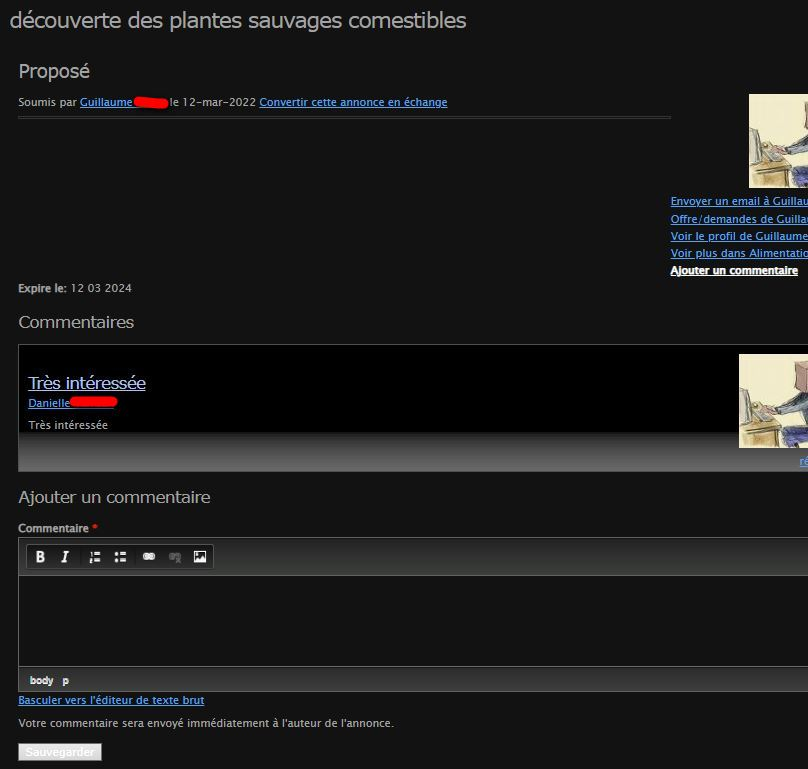
\includegraphics[width=.65\linewidth]{281-commentaires}
    \caption{Ajout de commentaires}
    \label{fig:commentaires}
\end{figure}
\begin{figure}
    \centering
    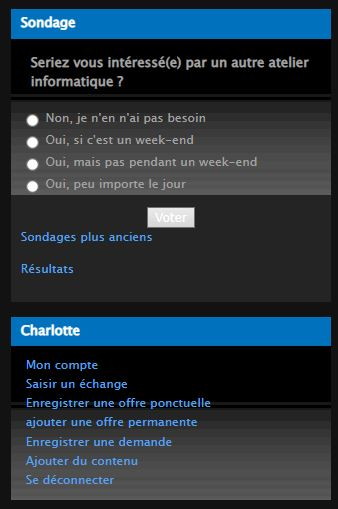
\includegraphics[width=.35\linewidth]{135-sondage}
    \caption{Bloc sondage sur la page <<~Actualités~>>}
    \label{fig:sondage}
\end{figure}

Le bloc du haut contient le menu utilisateur que nous avons vu en détails au chapitre \ref{chap:personnaliserCompte} <<~Personnaliser votre compte~>> (p. \pageref{chap:personnaliserCompte}) ainsi qu'à la section \ref{sec:menuUtilisateur2} <<~Menu utilisateur~>>, (p. \pageref{sec:menuUtilisateur2}) du présent chapitre.

\ssubsec{Commentaires}

\index{commentaires!liste des derniers}Dans le deuxième bloc de la colonne de droite, intitulé \noncliquables{Commentaires récents}, sont listés les cinq derniers commentaires publiés.

\index{commentaires!publier un|(}Lorsque vous consultez une annonce, vous avez la possibilité de poster un commentaire relatif à cette annonce; c’est également le cas pour certaines actualités ou d’autres documents. À la figure \ref{fig:commentaires}, un adhérent a proposé une sortie de découverte des plantes sauvages comestibles%
%%%
\footnote{Sans toutefois ajouter des précisions dans le cadre \noncliquables{Racontez votre histoire ...}!},
%%%
ensuite une adhérente a posté un commentaire disant qu'elle était intéressée; un autre commentaire pourrait être ajouté dans le cadre éponyme \noncliquables{Ajouter un commentaire}%
%%%
\footnote{Ici aussi il est possible de basculer vers l'édition de texte brut\index{editeur de texte brut@éditeur de texte brut} (voir p. \pageref{page:editeurTexteBrut})}.
%%%

Comme toujours, pour terminer, cliquez  sur \autresliens{Sauvegarder}.


 \rem[s]{(1) Attention, les commentaires ne sont pas diffusés par courriel, évitez donc de les utiliser pour des informations que vous souhaitez communiquer à l’ensemble des membres car nombreux sont ceux qui ne se connectent jamais sur le site et se contentent des courriels reçus.
 (2) Le lien \autresliens{Convertir cette annonce en échange} visible à la figure \ref{fig:commentaires} n'est pas utilisé au \CdS.}
 \index{commentaires!publier un|)}

 \ssubsec{Sondage}\index{sondage|(}
 
 Il est parfois utile, p.ex. avant de planifier une activité, une réunion, etc. de procéder à un sondage auprès des adhérent(e)s. Dans ce cas, la question posée et les cases de réponse apparaîtront dans un bloc qui prendra la place du menu utilisateur, ce dernier étant décalé vers le bas (voir Fig. \ref{fig:sondage})%
 %%%
 \footnote{Le bloc \noncliquables{Sondage} n'est présent que sur la page <<~Actualités~>> ou \index{page d'accueil}page d'accueil, sur les autres pages, le menu utilisateur est à sa place normale.}.
 %%%
 \index{sondage|)}

 Lorsque vous répondez à un sondage, n'oubliez pas de cliquer sur \autresliens{Voter}.

\subsec{Champ de recherche}\index{bloc!de recherche}

Tout en haut à droite, sous le menu secondaire, figure un champ de recherche (techniquement, il s’agit d’un autre bloc). Cet outil est rarement utilisé par les membres. Vous pouvez le supprimer (chapitre \ref{chap:personnaliserCompte}, section \og{}Supprimer l'affichage de certains blocs\fg.).

\subsec{Questionnaire}
\index{Questionnaire}

\index{organiser une activite@organiser une activité|(}
Par souci de complétude, ajoutons un dernier type de champ, le <<~Questionnaire~>> ou <<~Formulaire de contact~>>. Supposons une activité nécessitant une inscription --- pour connaître le nombre de participants, leurs attentes, leur condition physique, etc. L'organisatrice ou l'organisateur de l'activité peut demander à un membre du Comité (voir la liste p. \pageref{sec:comite}) de mettre en place un questionnaire publié sur le site. Pour l'instant, ceci n'a jamais été utilisé au \CdS, mais il est utile de savoir que c'est possible.

Si besoin, cette section sera développée dans une édition ultérieure de ce tutoriel.
\index{organiser une activite@organiser une activité|)}
